% Options for packages loaded elsewhere
\PassOptionsToPackage{unicode}{hyperref}
\PassOptionsToPackage{hyphens}{url}
\PassOptionsToPackage{dvipsnames,svgnames*,x11names*}{xcolor}
%
\documentclass[
  oneside]{krantz}
\usepackage{lmodern}
\usepackage{amssymb,amsmath}
\usepackage{ifxetex,ifluatex}
\ifnum 0\ifxetex 1\fi\ifluatex 1\fi=0 % if pdftex
  \usepackage[T1]{fontenc}
  \usepackage[utf8]{inputenc}
  \usepackage{textcomp} % provide euro and other symbols
\else % if luatex or xetex
  \usepackage{unicode-math}
  \defaultfontfeatures{Scale=MatchLowercase}
  \defaultfontfeatures[\rmfamily]{Ligatures=TeX,Scale=1}
\fi
% Use upquote if available, for straight quotes in verbatim environments
\IfFileExists{upquote.sty}{\usepackage{upquote}}{}
\IfFileExists{microtype.sty}{% use microtype if available
  \usepackage[]{microtype}
  \UseMicrotypeSet[protrusion]{basicmath} % disable protrusion for tt fonts
}{}
\makeatletter
\@ifundefined{KOMAClassName}{% if non-KOMA class
  \IfFileExists{parskip.sty}{%
    \usepackage{parskip}
  }{% else
    \setlength{\parindent}{0pt}
    \setlength{\parskip}{6pt plus 2pt minus 1pt}}
}{% if KOMA class
  \KOMAoptions{parskip=half}}
\makeatother
\usepackage{xcolor}
\IfFileExists{xurl.sty}{\usepackage{xurl}}{} % add URL line breaks if available
\IfFileExists{bookmark.sty}{\usepackage{bookmark}}{\usepackage{hyperref}}
\hypersetup{
  pdftitle={MTXXXX: Some stats},
  pdfauthor={L. Scott-Hayward and JJ Valletta},
  colorlinks=true,
  linkcolor=Maroon,
  filecolor=Maroon,
  citecolor=Blue,
  urlcolor=Blue,
  pdfcreator={LaTeX via pandoc}}
\urlstyle{same} % disable monospaced font for URLs
\usepackage{color}
\usepackage{fancyvrb}
\newcommand{\VerbBar}{|}
\newcommand{\VERB}{\Verb[commandchars=\\\{\}]}
\DefineVerbatimEnvironment{Highlighting}{Verbatim}{commandchars=\\\{\}}
% Add ',fontsize=\small' for more characters per line
\usepackage{framed}
\definecolor{shadecolor}{RGB}{248,248,248}
\newenvironment{Shaded}{\begin{snugshade}}{\end{snugshade}}
\newcommand{\AlertTok}[1]{\textcolor[rgb]{0.94,0.16,0.16}{#1}}
\newcommand{\AnnotationTok}[1]{\textcolor[rgb]{0.56,0.35,0.01}{\textbf{\textit{#1}}}}
\newcommand{\AttributeTok}[1]{\textcolor[rgb]{0.77,0.63,0.00}{#1}}
\newcommand{\BaseNTok}[1]{\textcolor[rgb]{0.00,0.00,0.81}{#1}}
\newcommand{\BuiltInTok}[1]{#1}
\newcommand{\CharTok}[1]{\textcolor[rgb]{0.31,0.60,0.02}{#1}}
\newcommand{\CommentTok}[1]{\textcolor[rgb]{0.56,0.35,0.01}{\textit{#1}}}
\newcommand{\CommentVarTok}[1]{\textcolor[rgb]{0.56,0.35,0.01}{\textbf{\textit{#1}}}}
\newcommand{\ConstantTok}[1]{\textcolor[rgb]{0.00,0.00,0.00}{#1}}
\newcommand{\ControlFlowTok}[1]{\textcolor[rgb]{0.13,0.29,0.53}{\textbf{#1}}}
\newcommand{\DataTypeTok}[1]{\textcolor[rgb]{0.13,0.29,0.53}{#1}}
\newcommand{\DecValTok}[1]{\textcolor[rgb]{0.00,0.00,0.81}{#1}}
\newcommand{\DocumentationTok}[1]{\textcolor[rgb]{0.56,0.35,0.01}{\textbf{\textit{#1}}}}
\newcommand{\ErrorTok}[1]{\textcolor[rgb]{0.64,0.00,0.00}{\textbf{#1}}}
\newcommand{\ExtensionTok}[1]{#1}
\newcommand{\FloatTok}[1]{\textcolor[rgb]{0.00,0.00,0.81}{#1}}
\newcommand{\FunctionTok}[1]{\textcolor[rgb]{0.00,0.00,0.00}{#1}}
\newcommand{\ImportTok}[1]{#1}
\newcommand{\InformationTok}[1]{\textcolor[rgb]{0.56,0.35,0.01}{\textbf{\textit{#1}}}}
\newcommand{\KeywordTok}[1]{\textcolor[rgb]{0.13,0.29,0.53}{\textbf{#1}}}
\newcommand{\NormalTok}[1]{#1}
\newcommand{\OperatorTok}[1]{\textcolor[rgb]{0.81,0.36,0.00}{\textbf{#1}}}
\newcommand{\OtherTok}[1]{\textcolor[rgb]{0.56,0.35,0.01}{#1}}
\newcommand{\PreprocessorTok}[1]{\textcolor[rgb]{0.56,0.35,0.01}{\textit{#1}}}
\newcommand{\RegionMarkerTok}[1]{#1}
\newcommand{\SpecialCharTok}[1]{\textcolor[rgb]{0.00,0.00,0.00}{#1}}
\newcommand{\SpecialStringTok}[1]{\textcolor[rgb]{0.31,0.60,0.02}{#1}}
\newcommand{\StringTok}[1]{\textcolor[rgb]{0.31,0.60,0.02}{#1}}
\newcommand{\VariableTok}[1]{\textcolor[rgb]{0.00,0.00,0.00}{#1}}
\newcommand{\VerbatimStringTok}[1]{\textcolor[rgb]{0.31,0.60,0.02}{#1}}
\newcommand{\WarningTok}[1]{\textcolor[rgb]{0.56,0.35,0.01}{\textbf{\textit{#1}}}}
\usepackage{longtable,booktabs}
% Correct order of tables after \paragraph or \subparagraph
\usepackage{etoolbox}
\makeatletter
\patchcmd\longtable{\par}{\if@noskipsec\mbox{}\fi\par}{}{}
\makeatother
% Allow footnotes in longtable head/foot
\IfFileExists{footnotehyper.sty}{\usepackage{footnotehyper}}{\usepackage{footnote}}
\makesavenoteenv{longtable}
\usepackage{graphicx,grffile}
\makeatletter
\def\maxwidth{\ifdim\Gin@nat@width>\linewidth\linewidth\else\Gin@nat@width\fi}
\def\maxheight{\ifdim\Gin@nat@height>\textheight\textheight\else\Gin@nat@height\fi}
\makeatother
% Scale images if necessary, so that they will not overflow the page
% margins by default, and it is still possible to overwrite the defaults
% using explicit options in \includegraphics[width, height, ...]{}
\setkeys{Gin}{width=\maxwidth,height=\maxheight,keepaspectratio}
% Set default figure placement to htbp
\makeatletter
\def\fps@figure{htbp}
\makeatother
\setlength{\emergencystretch}{3em} % prevent overfull lines
\providecommand{\tightlist}{%
  \setlength{\itemsep}{0pt}\setlength{\parskip}{0pt}}
\setcounter{secnumdepth}{5}
%============================================================================%
% St Andrews bookdown template 
% LaTeX preamble file
%============================================================================%
\renewcommand{\familydefault}{\sfdefault}
%============================================================================%
% Generic packages
%============================================================================%
\usepackage{booktabs}
\usepackage{longtable}
\usepackage{amsthm}

%============================================================================%
% Change Bibliography to References to match gitbook output
%============================================================================%
\renewcommand{\bibname}{References}

%============================================================================%
% Place all figures and tables after code chunk in PDF output
%============================================================================%
\usepackage{float}
\floatplacement{figure}{H}
\floatplacement{table}{H}

%============================================================================%
% Make index so we can print it later (see: afterbody.tex)
%============================================================================%
\usepackage{makeidx}
\makeindex

%============================================================================%
% Copied from Yihui's repo 
% https://github.com/rstudio/bookdown/tree/master/inst/examples
% First part to change spacing, second to cater for xetex latex engine
%============================================================================%
\makeatletter
\def\thm@space@setup{%
  \thm@preskip=8pt plus 2pt minus 4pt
  \thm@postskip=\thm@preskip
}
\makeatother

\ifxetex
  \usepackage{letltxmacro}
  \setlength{\XeTeXLinkMargin}{1pt}
  \LetLtxMacro\SavedIncludeGraphics\includegraphics
  \def\includegraphics#1#{% #1 catches optional stuff (star/opt. arg.)
    \IncludeGraphicsAux{#1}%
  }%
  \newcommand*{\IncludeGraphicsAux}[2]{%
    \XeTeXLinkBox{%
      \SavedIncludeGraphics#1{#2}%
    }%
  }%
\fi

%============================================================================%
% LaTeX macro to create task boxes
%============================================================================%
\usepackage{tcolorbox}
\tcbuselibrary{breakable}
\definecolor{taskCol}{HTML}{00539b}
\definecolor{taskCol1}{HTML}{007870}
\tcbset{colback=white,colframe=taskCol,arc=0mm}

% Trick to fool markdown into compiling
\newcommand{\bblockT}[2][Task]{\begin{tcolorbox}[title = #1 #2, parbox = false]}
\newcommand{\eblockT}{\end{tcolorbox}}
\newcommand{\bblockS}[2][Solution]{\begin{tcolorbox}[title = #1 #2, colframe=taskCol1, breakable, parbox = false]}
\newcommand{\eblockS}{\end{tcolorbox}}

% Add tabbed solutions environment
\newcommand{\bmp}{\begin{minipage}[c]{0.5\textwidth}}
\newcommand{\emp}{\end{minipage}}
\newcommand{\bblockST}[1]{\begin{tcolorbox}[title = #1, colframe=taskCol1, breakable, parbox = false]}
\newcommand{\eblockST}{\end{tcolorbox}}

% Set solution button link
\usepackage{tikz}

\newcommand{\buttonT}[1]{
    \begin{tikzpicture}
    \node[
        inner sep=5pt,
        draw=taskCol,
        fill=taskCol,
        rounded corners=2pt,
        text=white
    ] (c1) {#1};
    \end{tikzpicture}
}

\newcommand{\buttonS}[1]{
    \begin{tikzpicture}
    \node[
        inner sep=5pt,
        draw=taskCol1,
        fill=taskCol1,
        rounded corners=2pt,
        text=white
    ] (c1) {#1};
    \end{tikzpicture}
}
\newcommand{\colpageref}[1]{\hypersetup{linkcolor=white}\pageref{#1}}


%============================================================================%
% LaTeX to create coloured boxes
%============================================================================%

\usepackage{tcolorbox}

% \definecolor{backcolour}{HTML}{white}
\definecolor{framecolour}{HTML}{00539b}

\newtcolorbox{bluebox}{
  colback=white,
  colframe=framecolour,
  coltext=black,
  boxsep=5pt,
  arc=4pt}
  
\definecolor{framegreen}{HTML}{006962}
  
\newtcolorbox{greenbox}{
  colback=white,
  colframe=framegreen,
  coltext=black,
  boxsep=5pt,
  arc=4pt}

\definecolor{framecolour}{HTML}{00539b}
\definecolor{blueback}{HTML}{EEEEFF}

\newtcolorbox{palebluebox}{
  colback=blueback,
  colframe=framecolour,
  coltext=black,
  boxsep=5pt,
  arc=4pt}
\usepackage[]{natbib}
\bibliographystyle{apalike}

\title{MTXXXX: Some stats}
\author{\href{lass@st-andrews.ac.uk}{L. Scott-Hayward} and \href{jjv1@st-andrews.ac.uk}{JJ Valletta}}
\date{02 February 2021}

\usepackage{amsthm}
\newtheorem{theorem}{Theorem}[chapter]
\newtheorem{lemma}{Lemma}[chapter]
\newtheorem{corollary}{Corollary}[chapter]
\newtheorem{proposition}{Proposition}[chapter]
\newtheorem{conjecture}{Conjecture}[chapter]
\theoremstyle{definition}
\newtheorem{definition}{Definition}[chapter]
\theoremstyle{definition}
\newtheorem{example}{Example}[chapter]
\theoremstyle{definition}
\newtheorem{exercise}{Exercise}[chapter]
\theoremstyle{remark}
\newtheorem*{remark}{Remark}
\newtheorem*{solution}{Solution}
\begin{document}
\maketitle

{
\hypersetup{linkcolor=}
\setcounter{tocdepth}{2}
\tableofcontents
}
\hypertarget{welcome}{%
\chapter*{Welcome}\label{welcome}}


Welcome to MTXXXX: Some stats!

An introductory-course in the field of statistical modelling in R. The focus will be on how to fit statistical models in R. The target audience is anyone who wants to learn how to fit linear models in R. The progression will be linear models, generalised linear models and linear mixed effects models.

\hypertarget{prerequisites}{%
\section*{Prerequisites}\label{prerequisites}}


\begin{itemize}
\tightlist
\item
  Programming basics in R
\item
  MTXXXX
\end{itemize}

\hypertarget{learning-outcomes}{%
\section*{Learning outcomes}\label{learning-outcomes}}


\begin{itemize}
\tightlist
\item
  Understand the key concepts and terminology used in statistical modelling
\item
  Use R to fit linear, generalised linear and mixed effect models in R
\item
  Recognise practical issues with fitting these models
\item
  Checking model fit
\item
  Perform model comparisons
\end{itemize}

\hypertarget{recommended-reading}{%
\section*{Recommended reading}\label{recommended-reading}}


I highly recommend the following books:

\begin{itemize}
\tightlist
\item
  \href{https://www.wiley.com/en-gb/Statistics\%3A+An+Introduction+using+R-p-9780470022986}{Statistics: An Introduction using R}
\item
  \href{https://www.crcpress.com/Linear-Models-with-R/Faraway/p/book/9781439887332}{Linear models with R}
\end{itemize}

\hypertarget{data-files}{%
\section*{Data files}\label{data-files}}


All data files can be found on Moodle.

\hypertarget{assessment}{%
\section*{Assessment}\label{assessment}}


80\% written exam and 20\% \textbf{individual} coursework

\hypertarget{lateness-policy}{%
\section*{Lateness policy}\label{lateness-policy}}


The School has a lateness \href{https://www.st-andrews.ac.uk/maths/current/ug/information/latepenalties/}{policy}. The standard policy is an initial penalty of 15\% of the maximum available mark, then a further 5\% per 8-hour period, or part thereof for work submitted late without good reason.

\hypertarget{work-submitted-late-for-good-reason}{%
\section*{Work submitted late for good reason}\label{work-submitted-late-for-good-reason}}


If students have a justified reason for submitting work late, then the various University's policies relating to extenuating circumstances apply. In these circumstances, students must as soon as possible submit a self-certificate of absence and contact the relevant member of School (usually the module coordinator). You will then be advised whether further documentation is required and what format this documentation will take.

\hypertarget{acknowledgements}{%
\section*{Acknowledgements}\label{acknowledgements}}


We are indebted to all the statisticians who made some stats possible.

\hypertarget{intro}{%
\chapter{Introduction}\label{intro}}

The \href{https://bookdown.org/yihui/bookdown/}{\texttt{bookdown}} package can be installed from CRAN or Github:

\begin{Shaded}
\begin{Highlighting}[]
\KeywordTok{install.packages}\NormalTok{(}\StringTok{"bookdown"}\NormalTok{)}
\CommentTok{# or the development version}
\CommentTok{# devtools::install_github("rstudio/bookdown")}
\end{Highlighting}
\end{Shaded}

\href{https://bookdown.org/yihui/bookdown/}{\texttt{bookdown}} is a tool for combining multiple R Markdown documents into a single book.

Each \texttt{.Rmd} file contains one and only one chapter, and a chapter is defined by the first-level heading \texttt{\#} (e.g.~\texttt{\#\ Introduction}).
To learn more about R Markdown read \href{https://bookdown.org/yihui/rmarkdown/}{R Markdown: The Definitive Guide}.

To compile to PDF, you need to have LaTeX installed on your machine. \texttt{xelatex} and \texttt{lualatex} are recommended as they support Unicode better
(see \href{https://tex.stackexchange.com/questions/3393/what-is-xetex-exactly-and-why-should-i-use-it}{here} and \href{https://tex.stackexchange.com/questions/36/differences-between-luatex-context-and-xetex}{here} for details).
For a lightweight LaTeX installation one can use \href{https://yihui.org/tinytex/}{\texttt{TinyTeX}} (which includes \texttt{xelatex}).

You can label chapter and section titles using the \texttt{\{\#label\}} syntax. For example \texttt{\#\ Introduction\ \{\#intro\}} assigns the label \texttt{intro} to the introductory chapter.
We can then reference the chapter using the \texttt{\textbackslash{}@ref(label)} syntax. For example, Chapter \texttt{\textbackslash{}@ref(intro)} renders as Chapter \ref{intro}.

\hypertarget{figures-and-tables}{%
\section{Figures and Tables}\label{figures-and-tables}}

Figures and tables with captions are placed in \texttt{figure} and \texttt{table} environments, respectively.

Reference a figure by its code chunk label with the \texttt{fig:} prefix. For example, Figure \texttt{\textbackslash{}@ref(fig:nice-fig)} renders as Figure \ref{fig:nice-fig}.

\begin{Shaded}
\begin{Highlighting}[]
\KeywordTok{par}\NormalTok{(}\DataTypeTok{mar =} \KeywordTok{c}\NormalTok{(}\DecValTok{4}\NormalTok{, }\DecValTok{4}\NormalTok{, }\FloatTok{.1}\NormalTok{, }\FloatTok{.1}\NormalTok{))}
\KeywordTok{plot}\NormalTok{(pressure, }\DataTypeTok{type =} \StringTok{'b'}\NormalTok{, }\DataTypeTok{pch =} \DecValTok{19}\NormalTok{)}
\end{Highlighting}
\end{Shaded}

\begin{figure}

{\centering 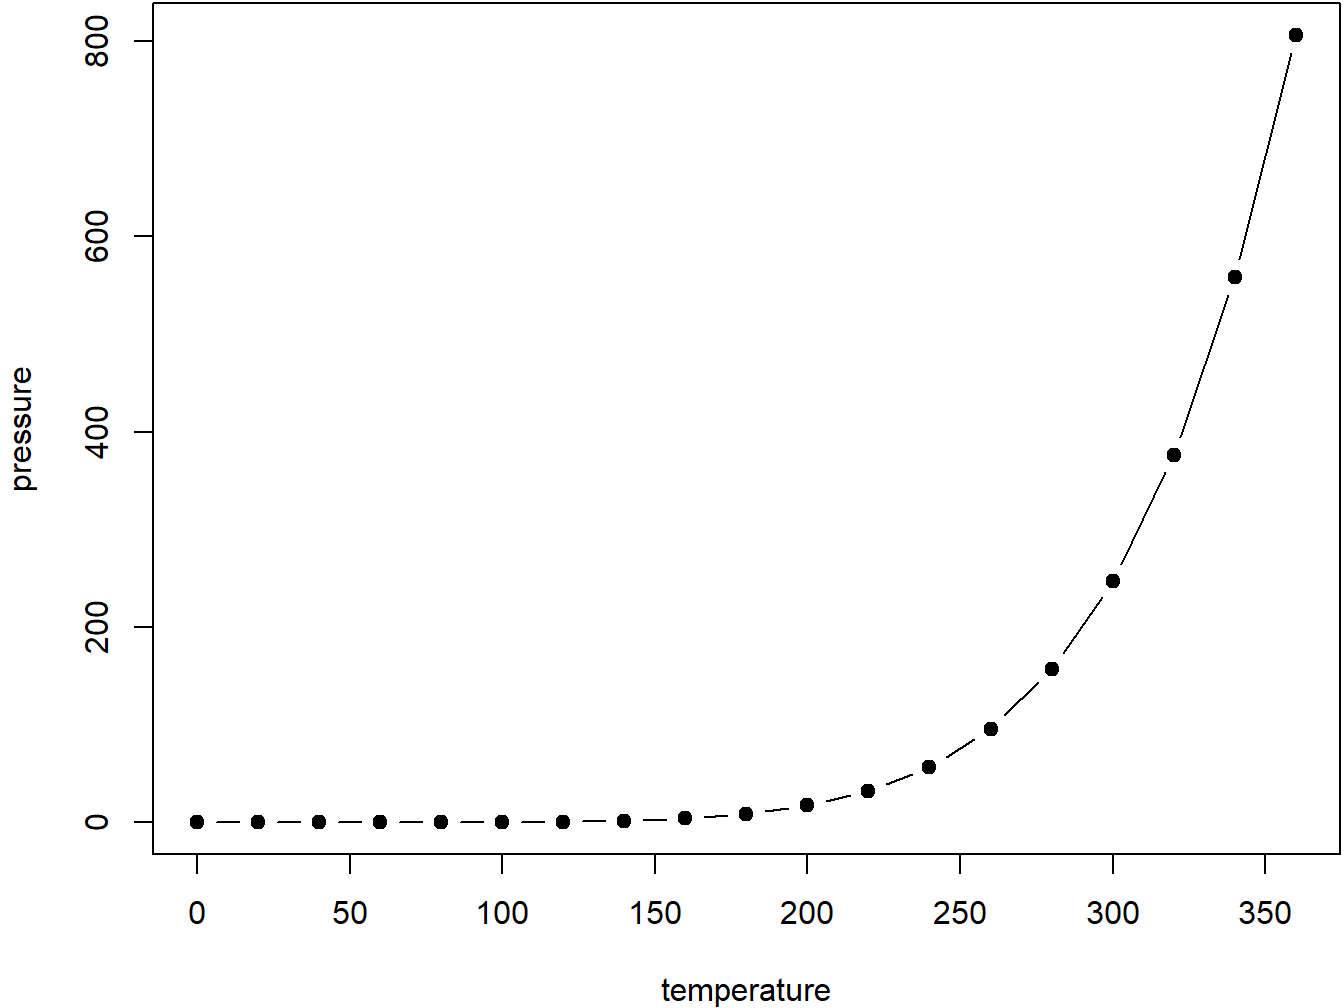
\includegraphics[width=0.8\linewidth]{StAndrewsTemplate_files/figure-latex/nice-fig-1} 

}

\caption{Here is a nice figure!}\label{fig:nice-fig}
\end{figure}

Similarly, tables generated by \texttt{knitr::kable()} can be referenced by their code chunk label with the \texttt{tab:} prefix. For example, Table \texttt{\textbackslash{}@ref(tab:nice-tab)} renders as Table \ref{tab:nice-tab}.

\begin{Shaded}
\begin{Highlighting}[]
\NormalTok{knitr}\OperatorTok{::}\KeywordTok{kable}\NormalTok{(}
  \KeywordTok{head}\NormalTok{(iris, }\DecValTok{10}\NormalTok{), }\DataTypeTok{caption =} \StringTok{'Here is a nice table!'}\NormalTok{,}
  \DataTypeTok{booktabs =} \OtherTok{TRUE}
\NormalTok{)}
\end{Highlighting}
\end{Shaded}

\begin{table}

\caption{\label{tab:nice-tab}Here is a nice table!}
\centering
\begin{tabular}[t]{rrrrl}
\toprule
Sepal.Length & Sepal.Width & Petal.Length & Petal.Width & Species\\
\midrule
5.1 & 3.5 & 1.4 & 0.2 & setosa\\
4.9 & 3.0 & 1.4 & 0.2 & setosa\\
4.7 & 3.2 & 1.3 & 0.2 & setosa\\
4.6 & 3.1 & 1.5 & 0.2 & setosa\\
5.0 & 3.6 & 1.4 & 0.2 & setosa\\
\addlinespace
5.4 & 3.9 & 1.7 & 0.4 & setosa\\
4.6 & 3.4 & 1.4 & 0.3 & setosa\\
5.0 & 3.4 & 1.5 & 0.2 & setosa\\
4.4 & 2.9 & 1.4 & 0.2 & setosa\\
4.9 & 3.1 & 1.5 & 0.1 & setosa\\
\bottomrule
\end{tabular}
\end{table}

You can also do a text reference for a figure caption which is useful if you want to include a mathematical expression and/or caption is very long. The syntax is ``\texttt{(ref:label)} Some text which can include equations''.



\begin{Shaded}
\begin{Highlighting}[]
\KeywordTok{par}\NormalTok{(}\DataTypeTok{mar =} \KeywordTok{c}\NormalTok{(}\DecValTok{4}\NormalTok{, }\DecValTok{4}\NormalTok{, }\FloatTok{.1}\NormalTok{, }\FloatTok{.1}\NormalTok{))}
\KeywordTok{plot}\NormalTok{(pressure, }\DataTypeTok{type =} \StringTok{'b'}\NormalTok{, }\DataTypeTok{pch =} \DecValTok{19}\NormalTok{, }\DataTypeTok{col=}\DecValTok{2}\NormalTok{)}
\end{Highlighting}
\end{Shaded}

\begin{figure}

{\centering 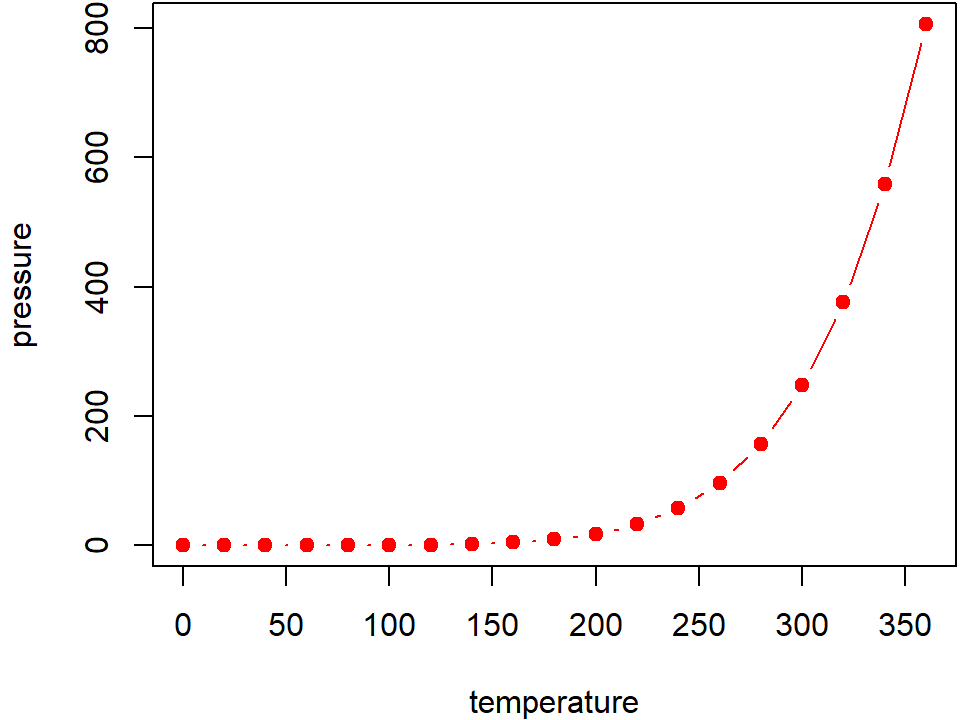
\includegraphics[width=0.8\linewidth]{StAndrewsTemplate_files/figure-latex/nice-fig2-1} 

}

\caption{A text reference with a mathematical expression \(y_i=\beta_0 + \beta_1x_i + \epsilon_i\) and \(\epsilon_i \sim \mathcal{N}(0, \sigma^2)\).}\label{fig:nice-fig2}
\end{figure}

You can write citations, too. For example, we are using the \textbf{bookdown} package \citep{R-bookdown} in this sample book, which was built on top of R Markdown and \textbf{knitr} \citep{xie2015}.

\hypertarget{equations}{%
\section{Equations}\label{equations}}

\begin{verbatim}
\begin{equation} 
  f\left(k\right) = \binom{n}{k} p^k\left(1-p\right)^{n-k}
  \label{eq:binom}
\end{equation} 
\end{verbatim}

renders as:

\begin{equation} 
  f\left(k\right) = \binom{n}{k} p^k\left(1-p\right)^{n-k}
  \label{eq:binom}
\end{equation}

You may refer to it using \texttt{\textbackslash{}@ref(eq:binom)} which renders as \eqref{eq:binom}.

Please make sure equations \index{equations} without labels are not numbered by either using the \texttt{equation*} environment or adding \texttt{\textbackslash{}nonumber} or \texttt{\textbackslash{}notag} to your equations. The same rules apply to other math environments. For aligning multiple equations, \texttt{align} is the preferred environment. For \url{example:/index\%7Balign\%7D}

\begin{verbatim}
\begin{align} 
g(X_{n}) & = g(\theta)+g'({\tilde{\theta}})(X_{n}-\theta) \notag \\
\sqrt{n}[g(X_{n})-g(\theta)] & = g'\left({\tilde{\theta}}\right) 
\sqrt{n}[X_{n}-\theta]\label{eq:align} \\
\end{align} 
\end{verbatim}

renders as

\begin{align} 
g(X_{n}) & = g(\theta)+g'({\tilde{\theta}})(X_{n}-\theta) \notag \\
\sqrt{n}[g(X_{n})-g(\theta)] & = g'\left({\tilde{\theta}}\right) 
\sqrt{n}[X_{n}-\theta]\label{eq:align} \\
\end{align}

Use split to have multiple lines with one equation reference. For example:

\begin{verbatim}
\begin{equation} 
\begin{split}
\mathrm{Var}(\hat{\beta}) & =\mathrm{Var}((X'X)^{-1}X'y)\\
 & =(X'X)^{-1}X'\mathrm{Var}(y)((X'X)^{-1}X')'\\
 & =(X'X)^{-1}X'\mathrm{Var}(y)X(X'X)^{-1}\\
 & =(X'X)^{-1}X'\sigma^{2}IX(X'X)^{-1}\\
 & =(X'X)^{-1}\sigma^{2}
\end{split}
\label{eq:var-beta}
\end{equation} 
\end{verbatim}

renders as

\begin{equation} 
\begin{split}
\mathrm{Var}(\hat{\beta}) & =\mathrm{Var}((X'X)^{-1}X'y)\\
 & =(X'X)^{-1}X'\mathrm{Var}(y)((X'X)^{-1}X')'\\
 & =(X'X)^{-1}X'\mathrm{Var}(y)X(X'X)^{-1}\\
 & =(X'X)^{-1}X'\sigma^{2}IX(X'X)^{-1}\\
 & =(X'X)^{-1}\sigma^{2}
\end{split}
\label{eq:var-beta}
\end{equation}

\hypertarget{examples}{%
\section{Examples}\label{examples}}

Using the \texttt{example} environment. For example: \index{confidence intervals}

\begin{verbatim}
``{example, eg1, name='Confidence intervals using the Normal approximation.'}
\begin{alignat*}{2}
-z_{\alpha/2} \leq{} & \;\;\;Z & \leq{} & z_{\alpha/2} \\
-z_{\alpha/2} \leq{} & \frac{\hat{\mu}-\mu}{\frac{\sigma}{\sqrt{n}}} & \leq{} & z_{\alpha/2}\\
\hat{\mu} - z_{\alpha/2}\frac{\sigma}{\sqrt{n}} \leq{} & \;\;\;\mu & \leq{} & \hat{\mu} + z_{\alpha/2}\frac{\sigma}{\sqrt{n}}
\end{alignat*}
``
\end{verbatim}

renders as

\begin{example}[Confidence intervals using the Normal approximation.]
\protect\hypertarget{exm:eg1}{}{\label{exm:eg1} \iffalse (Confidence intervals using the Normal approximation.) \fi{} }\begin{alignat*}{2}
-z_{\alpha/2} \leq{} & \;\;\;Z & \leq{} & z_{\alpha/2} \\
-z_{\alpha/2} \leq{} & \frac{\hat{\mu}-\mu}{\frac{\sigma}{\sqrt{n}}} & \leq{} & z_{\alpha/2}\\
\hat{\mu} - z_{\alpha/2}\frac{\sigma}{\sqrt{n}} \leq{} & \;\;\;\mu & \leq{} & \hat{\mu} + z_{\alpha/2}\frac{\sigma}{\sqrt{n}}
\end{alignat*}
\end{example}

We can reference the example by its code chunk label with the \texttt{exm:} prefix. For example, Example \texttt{\textbackslash{}@ref(exm:eg1)} renders as Example \ref{exm:eg1}.

There are also \texttt{theorem}, \texttt{lemma}, etc. environments. Full details can be found \href{https://bookdown.org/yihui/bookdown/markdown-extensions-by-bookdown.html}{here}.

You can also create blocks of text using the simple \texttt{\textgreater{}} without the need for a chunk. For example,

\begin{verbatim}
> **Aside**: using the model to predict outside of the range 
of the observed data is called **extrapolating**.
\end{verbatim}

renders as

\begin{quote}
\textbf{Aside}: using the model to predict outside of the range of the observed data is called \textbf{extrapolating}.
\end{quote}

\hypertarget{shiny-apps-and-html-widgets}{%
\section{Shiny apps and HTML widgets}\label{shiny-apps-and-html-widgets}}

You can add \href{https://bookdown.org/yihui/bookdown/web-pages-and-shiny-apps.html}{Shiny apps} and \href{https://bookdown.org/yihui/bookdown/html-widgets.html}{HTML widgets} to your book.

For example, using the \texttt{knitr::include\_app(...)} function we can embed a Shiny app that is hosted somewhere else.
Note that this app renders as an interactive panel in the web book and a static screenshot in the PDF. For the PDF image to work properly, make sure you include \texttt{dev=\textquotesingle{}png\textquotesingle{}} in the chunk header. You can then click on either the image or the link in the caption to live view the app.

\begin{verbatim}
``{r myshiny, echo=FALSE, screenshot.opts=list(delay=3), dev='png',fig.cap='An example of a shiny app. You can see a live version \href{https://lindesaysh.shinyapps.io/faithfulshiny/}{here}'}
knitr::include_app("https://lindesaysh.shinyapps.io/faithfulshiny/", height='600px')
``
\end{verbatim}

renders as



\begin{figure}

{\centering \href{https://lindesaysh.shinyapps.io/faithfulshiny/}{\includegraphics{StAndrewsTemplate_files/figure-latex/myshiny-1} }

}

\caption{An example of a shiny app. You can see a live version \href{https://lindesaysh.shinyapps.io/faithfulshiny/}{here}}\label{fig:myshiny}
\end{figure}

\hypertarget{bellsandwhistles}{%
\chapter{Bells and Whistles}\label{bellsandwhistles}}

Chapter \ref{intro} briefly introduces the basic features of R Markdown and bookdown. For full details please refer to:

\begin{itemize}
\tightlist
\item
  \href{https://bookdown.org/yihui/rmarkdown/}{R Markdown: The Definitive Guide}
\item
  \href{https://bookdown.org/yihui/bookdown/}{bookdown: Authoring Books and Technical Documents with R Markdown}
\end{itemize}

In this Chapter we are going to introduce \emph{extra} features/environments exclusive to the St Andrews template. Big thanks to \href{https://github.com/tjmckinley/RtutorialSkeleton}{TJ McKinley} for sharing with us the code for the task and solution features.

\hypertarget{task-and-solution-block}{%
\section{Task and solution block}\label{task-and-solution-block}}

The \texttt{task} block can be used to set exercises for the students. The \texttt{solution} block reveals the answer to the student (if enabled; more on that later). For the gitbook/HTML version
there is a toggle button \texttt{Show\ Solution} that reveals the answer. In the PDF version, there is a hyperlink to take the reader to the solutions, which are in the appendix. There is also a link to get back to the place in the text from the appendix.

The \texttt{task} block is used as follows. For example:

\begin{verbatim}
```{task}
Here is a task written in **markdown**.
```
\end{verbatim}

which renders as:

\hypertarget{tsk1}{}\bblockT[Task]{\phantomsection\label{sol1}1}

Here is a task written in \textbf{markdown}.
\eblockT

You can include chunks within the \texttt{task} chunk, but you need to use double backticks \emph{within} the chunk, and leave carriage returns around the internal chunk. For example:

\begin{verbatim}

```{task}

``{r}
x <- 2 + 2
x
``

```
\end{verbatim}

which renders as:

\hypertarget{tsk2}{}\bblockT[Task]{\phantomsection\label{sol2}2}

\begin{Shaded}
\begin{Highlighting}[]
\NormalTok{x <-}\StringTok{ }\DecValTok{2} \OperatorTok{+}\StringTok{ }\DecValTok{2}
\NormalTok{x}
\end{Highlighting}
\end{Shaded}

\begin{verbatim}
## [1] 4
\end{verbatim}

\eblockT

Be careful to have suitable carriage returns around e.g.~\texttt{enumerate} or \texttt{itemize} environments inside the chunk also. For example:

\begin{verbatim}

```{task}
Here is a list:
1. item 1
2. item 2
```
\end{verbatim}

will not render nicely. But

\begin{verbatim}

```{task}
Here is a list:

1. item 1
2. item 2

```
\end{verbatim}

will:

\hypertarget{tsk3}{}\bblockT[Task]{\phantomsection\label{sol3}3}

Here is a list:

\begin{enumerate}
\def\labelenumi{\arabic{enumi}.}
\tightlist
\item
  item 1
\item
  item 2
\end{enumerate}

\eblockT

The \texttt{solution} chunk works in the same way, and the numbers will follow the previous \texttt{task} chunk (so you can set tasks without solutions). For example:

\begin{verbatim}

```{task}
Add 2 and 2 together
```

```{solution}

``{r}
2 + 2
``

```
\end{verbatim}

gives:

\hypertarget{tsk4}{}\bblockT[Task]{\phantomsection\label{sol4}4}

Add 2 and 2 together
\eblockT

\hyperlink{sol4}{\buttonS{Show Solution on P\colpageref{tsk4}}}

\hypertarget{different-task-and-solution-titles}{%
\section{Different task and solution titles}\label{different-task-and-solution-titles}}

\texttt{task} and \texttt{solution} boxes can be given different names using the \texttt{title} option (these can be set globally if preferred). For example:

\begin{verbatim}

```{task, title = "Question"}
Produce a scatterplot of `mpg` against `hp`. What does the relationship look like?
```

```{solution, title = "Answer"}

``{r}
plot(hp ~ mpg, data = mtcars, 
  pch=19, col='darkgrey')
``

```
\end{verbatim}

renders as:

\hypertarget{tsk5}{}\bblockT[Question]{\phantomsection\label{sol5}5}

Produce a scatterplot of \texttt{mpg} against \texttt{hp}. What does the relationship look like?
\eblockT

\hyperlink{sol5}{\buttonS{Show Answer on P\colpageref{tsk5}}}

\hypertarget{two-tabbed-solution}{%
\section{Two-tabbed solution}\label{two-tabbed-solution}}

You can have a task with \textbf{two} different solutions side-by-side, using the \texttt{multCode\ =\ T} option to the solution box. For example, you may want to show a solution using both base \texttt{R} and \texttt{tidyverse}. Here the two tabs are separated by four consecutive hashes: \texttt{\#\#\#\#}, and the \texttt{titles} option gives the tab titles (these can be set globally if preferred). For example:

\begin{verbatim}

```{task}
Produce a scatterplot of `mpg` against `hp`. What does the relationship look like?
```

```{solution, multCode=T, titles = c("Base R", "tidyverse")}

``{r, fig.height=6, fig.width=6, out.width = "60%"}
plot(hp ~ mpg, data = mtcars,
     pch=19, col='darkgrey')
``

The plot suggests that a linear relationship might exist between the two variables. 
So we can proceed by fitting a linear model in R.

####

``{r, fig.height=6, fig.width=6, out.width = "60%"}
ggplot(mtcars) +
    geom_point(aes(x = mpg, y = hp))
``

The plot suggests that a linear relationship might exist between the two variables. 
So we can proceed by fitting a linear model in R.
    
```
\end{verbatim}

will render as:

\hypertarget{tsk6}{}\bblockT[Task]{\phantomsection\label{sol6}6}

Produce a scatterplot of \texttt{mpg} against \texttt{hp}. What does the relationship look like?
\eblockT

\hyperlink{sol6}{\buttonS{Show Solution on P\colpageref{tsk6}}}

\hypertarget{multi-tabbed-options}{%
\section{Multi-tabbed options}\label{multi-tabbed-options}}

You can also have just the multicode part (not embedded within the solution panel.). These appear side-by-side in the PDF document. Note that currently you can only have \textbf{two} tabs. For example:

\begin{verbatim}

```{multCode, titles=c('Part A', 'Part B')}

Two options: 

* Option 1 - This is some text for part A

####

Two options:
    
* Option 2 - This is some text for part B

```
\end{verbatim}

will typeset to:

\bmp
\bblockST{Part A}

Two options:

\begin{itemize}
\tightlist
\item
  Option 1 - This is some text for part A
\end{itemize}

\eblockST
\emp
\hspace{0.01\textwidth}
\bmp\bblockST{Part B}

Two options:

\begin{itemize}
\tightlist
\item
  Option 2 - This is some text for part B
\end{itemize}

\eblockST
\emp

\hypertarget{task-with-held-solutions}{%
\section{Task with held solutions}\label{task-with-held-solutions}}

In the solution chunk header, if \texttt{renderSol=FALSE} then the solutions are not rendered as part of the book. For example:

\begin{verbatim}

```{task, title='Task (solution hidden)'}
Produce a scatterplot of `mpg` against `hp`. What does the relationship look like?
```

```{solution, renderSol=FALSE}

``{r}
plot(hp ~ mpg, data = mtcars, 
  pch=19, col='darkgrey')
``

This is my solution which you will only see if `renderSol` is set to `TRUE`.

```
\end{verbatim}

will render as:

\hypertarget{tsk7}{}\bblockT[Task (solution hidden)]{\phantomsection\label{sol7}7}

Produce a scatterplot of \texttt{mpg} against \texttt{hp}. What does the relationship look like?
\eblockT

By default, in \texttt{\_setup.Rmd}, \texttt{renderSol} is set to \texttt{TRUE}. If one of your chapters is a tutorial/practical, and you want to release the answers later on in the course,
it can become tedious having to set \texttt{renderSol} to \texttt{FALSE} for every question.
Instead, you can override this default at the beginning of each chapter, so you can turn on/off the solutions, as follows:

\begin{verbatim}

``{r, include=F}
opts_chunk$set(renderSol=FALSE)
``
\end{verbatim}

\textbf{Note} that the chunk above changes everything after the chunk, so later chapters will retain this change unless you reset it.

\hypertarget{adding-boxes}{%
\section{Adding Boxes}\label{adding-boxes}}

Sometimes you may wish to add a box section to your notes. There are currently three different coloured boxes defined; green and blue with white backgrounds and blue with pale blue background. For example,

\begin{verbatim}
:::: {.greenbox data-latex=""}
This is an example of a green box.
::::

:::: {.bluebox data-latex=""}
This is an example of a blue box.
::::

:::: {.palebluebox data-latex=""}
This is an example of a blue box with pale blue background.
::::
\end{verbatim}

will render as:

\begin{greenbox}

This is an example of a green box.

\end{greenbox}

\begin{bluebox}

This is an example of a blue box.

\end{bluebox}

\begin{palebluebox}

This is an example of a blue box with pale blue background.

\end{palebluebox}

You can also give your box a title. You can use \texttt{:::} to denote a separate section inside the box:

\begin{verbatim}
:::: {.palebluebox data-latex=""}
::: {.center data-latex=""}
**This is my title**
:::

This is the contents of my box.

::::
\end{verbatim}

renders as

\begin{palebluebox}

\begin{center}

\textbf{This is my title}

\end{center}

This is the contents of my box.

\end{palebluebox}

You can add equations, figures, r-code etc to your boxes. For example:

\begin{verbatim}
:::: {.greenbox data-latex=""}
::: {.center data-latex=""}
**Things you can include**
:::

Equations: 
$$y = \beta_0 + \beta_1X$$

R-code:

```r
1+1
```

Figures:


Formatting:

+ **bold**
+ *italic*
    a) sub bullets

::::
\end{verbatim}

will render as:

\begin{greenbox}

\begin{center}

\textbf{Things you can include}

\end{center}

Equations:

\[y = \beta_0 + \beta_1X\]
R-code:

\begin{Shaded}
\begin{Highlighting}[]
\DecValTok{1}\OperatorTok{+}\DecValTok{1}
\end{Highlighting}
\end{Shaded}

\begin{verbatim}
## [1] 2
\end{verbatim}

Figures:

\begin{center}
\includegraphics[width=0.1\linewidth]{standard-vertical-black} \end{center}

Formatting:

\begin{itemize}
\tightlist
\item
  \textbf{bold}
\item
  \emph{italic}

  \begin{enumerate}
  \def\labelenumi{\alph{enumi})}
  \tightlist
  \item
    sub bullets
  \end{enumerate}
\end{itemize}

\end{greenbox}

The colour scheme for the boxes is defined in the following files:

\begin{itemize}
\tightlist
\item
  \texttt{style.css}. For html output, see the section ``Create colour scheme for boxes''
\item
  \texttt{preamble.tex}. For pdf output, see the section ``LaTeX to create coloured boxes''
\end{itemize}

For more information on these boxes and other custom blocks have a look at \href{https://bookdown.org/yihui/rmarkdown-cookbook/custom-blocks.html}{this section} of the R-Markdown Cookbook.

\hypertarget{final-words}{%
\chapter{Final Words}\label{final-words}}

This template contains several files with different extensions and may look daunting at first. However, unless you want to customise specific aspects of this template, you \emph{only} need to edit/add individual R Markdown files corresponding to each chapter of your course notes. Nevertheless, here's a brief description of each file in this template stratified by type.

\hypertarget{what-are-all-these-files-for}{%
\section{What are all these files for?}\label{what-are-all-these-files-for}}

\hypertarget{markdown-files}{%
\subsection*{Markdown files}\label{markdown-files}}


\begin{itemize}
\item
  \texttt{index.Rmd}: The \emph{only} non-optional file.

  \begin{enumerate}
  \def\labelenumi{\arabic{enumi}.}
  \tightlist
  \item
    Starts with a YAML configuration file to set the title, author, date and other build options.
  \end{enumerate}

\begin{Shaded}
\begin{Highlighting}[]
\PreprocessorTok{--- }
\FunctionTok{title}\KeywordTok{:}\AttributeTok{ }\StringTok{"MTXXXX: Some stats"}
\FunctionTok{description}\KeywordTok{:}\AttributeTok{ }\StringTok{"This is an example gitbook with some St Andrews styling."}
\FunctionTok{author}\KeywordTok{:}\AttributeTok{ }\StringTok{"[L. Scott-Hayward](lass@st-andrews.ac.uk) and [JJ Valletta](jjv1@st-andrews.ac.uk)"}
\FunctionTok{date}\KeywordTok{:}\AttributeTok{ }\StringTok{'02 February 2021'}
\FunctionTok{site}\KeywordTok{:}\AttributeTok{ bookdown::bookdown_site}
\FunctionTok{documentclass}\KeywordTok{:}\AttributeTok{ krantz}
\FunctionTok{classoption}\KeywordTok{:}\AttributeTok{ oneside}
\FunctionTok{bibliography}\KeywordTok{:}\AttributeTok{ }\KeywordTok{[}\AttributeTok{book.bib}\KeywordTok{,}\AttributeTok{ packages.bib}\KeywordTok{]}
\FunctionTok{biblio-style}\KeywordTok{:}\AttributeTok{ apalike}
\FunctionTok{link-citations}\KeywordTok{:}\AttributeTok{ }\CharTok{yes}
\FunctionTok{colorlinks}\KeywordTok{:}\AttributeTok{ }\CharTok{yes}
\PreprocessorTok{---}
\end{Highlighting}
\end{Shaded}

  \begin{enumerate}
  \def\labelenumi{\arabic{enumi}.}
  \setcounter{enumi}{1}
  \tightlist
  \item
    Sets the global \texttt{knitr} options. These options can be overridden at the start of each chapter if one wants each chapter to have its own default options.
  \end{enumerate}

\begin{verbatim}
``{r setup, echo=FALSE}
library(knitr)
## set knitr global options
opts_chunk$set(cache=F, tidy.opts=list(width.cutoff=55), tidy=F, 
               fig.align="center", fig.width=5, fig.height=5,
               multCode=F, renderTask=T, renderSol=T)
``
\end{verbatim}

  \begin{enumerate}
  \def\labelenumi{\arabic{enumi}.}
  \setcounter{enumi}{2}
  \tightlist
  \item
    Add \texttt{\_setup.Rmd} to the book.
  \end{enumerate}

\begin{verbatim}
``{r, child = "_setup.Rmd", include = F, purl = F, cache = F}
``
\end{verbatim}

  \begin{enumerate}
  \def\labelenumi{\arabic{enumi}.}
  \setcounter{enumi}{3}
  \tightlist
  \item
    Normal R Markdown. Typically contains the preface of your course notes, as shown in the template.
    Although it can be written as a separate \texttt{.Rmd} file for more modularity.
  \end{enumerate}

\begin{verbatim}
# Welcome {-}

Welcome to MTXXXX: Some stats!
...
\end{verbatim}

  \begin{enumerate}
  \def\labelenumi{\arabic{enumi}.}
  \setcounter{enumi}{4}
  \tightlist
  \item
    The last chunk of code in \texttt{index.Rmd} creates a BibTeX file to reference the packages used, see \texttt{packages.bib} for more details. This is optional.
  \end{enumerate}
\item
  \texttt{\_setup.Rmd}: This file specifies features/environments exclusive to this template; the task/solution block, multi-tabbed solutions, etc (see Chapter \ref{bellsandwhistles}).
  Do not edit this file!
\item
  \texttt{01-intro.Rmd} - \texttt{03-summary.Rmd}: These files contain all the content of your course notes. Each \texttt{.Rmd} file is a chapter and must begin with a single \texttt{\#} level header (e.g.~\texttt{\#\ Linear\ regression}). You can have as many files as you want. \texttt{.Rmd} files are added to the book in alphabetical order. It is therefore recommended to number the files in the order you'd like them to appear. Alternatively, use \texttt{\_bookdown.yml} to specify the precise order (more on that later).
\item
  \texttt{04-references.Rmd}: Appends references at the end of the gitbook/HTML book. You can edit the name of the file, but don't edit what's in it.
\item
  \texttt{05-ch\_appendix.Rmd}: Appends solutions at the end of the PDF file. You can edit the name of the file, but don't edit what's in it.
\item
  \texttt{README.md}: Primarily intended as a landing page for the \href{https://github.com/lindesaysh/StAndrewsTemplateBookdown}{Github repo} where this template is currently residing. This file can be safely deleted. Alternatively, if you don't use version control (like git), this file can be used to keep track of any major changes done to your course notes.
\end{itemize}

\hypertarget{yaml-files}{%
\subsection*{YAML files}\label{yaml-files}}


\href{https://en.wikipedia.org/wiki/YAML}{YAML} files are human-readable files typically used for configuration files.

\begin{itemize}
\tightlist
\item
  \texttt{\_bookdown.yml}: Overarching configuration file for the book; set book file name, output directory, etc. It allows you to choose which chapters to include under which build (gitbook/html or pdf/latex). This is particularly useful when you're working on a large number of chapters. Through the \texttt{rmd\_files} option you can choose to only compile the chapter you're currently working on, which reduces compilation time significantly.
\end{itemize}

\textbf{Note}: The \texttt{latex} option must have the \texttt{appendix.Rmd} file as its last entry (name of file is irrelevant). This ensures that the appendix is properly formatted for the solutions to the problems. This is \emph{only} needed for the PDF output; for gitbook/HTML, the task/solution block uses a toggle button instead.

\begin{Shaded}
\begin{Highlighting}[]
\FunctionTok{book_filename}\KeywordTok{:}\AttributeTok{ }\StringTok{"StAndrewsTemplate"}
\FunctionTok{language}\KeywordTok{:}
\AttributeTok{  }\FunctionTok{ui}\KeywordTok{:}
\AttributeTok{    }\FunctionTok{chapter_name}\KeywordTok{:}\AttributeTok{ }\StringTok{"Chapter "}
\FunctionTok{delete_merged_file}\KeywordTok{:}\AttributeTok{ }\CharTok{true}
\FunctionTok{rmd_files}\KeywordTok{:}
\AttributeTok{  }\FunctionTok{html}\KeywordTok{:}\AttributeTok{ }\KeywordTok{[}\StringTok{"index.Rmd"}\KeywordTok{,}\AttributeTok{ }\StringTok{"01-intro.Rmd"}\KeywordTok{,}\AttributeTok{ }\StringTok{"02-bellsandwhistles.Rmd"}\KeywordTok{,}\AttributeTok{ }\StringTok{"03-summary.Rmd"}\KeywordTok{,}\AttributeTok{ }\StringTok{"04-references.Rmd"}\KeywordTok{]}
\AttributeTok{  }\FunctionTok{latex}\KeywordTok{:}\AttributeTok{ }\KeywordTok{[}\StringTok{"index.Rmd"}\KeywordTok{,}\AttributeTok{ }\StringTok{"01-intro.Rmd"}\KeywordTok{,}\AttributeTok{ }\StringTok{"02-bellsandwhistles.Rmd"}\KeywordTok{,}\AttributeTok{ }\StringTok{"03-summary.Rmd"}\KeywordTok{,}\AttributeTok{  }\StringTok{"04-references.Rmd"}\KeywordTok{,}\AttributeTok{ }\StringTok{"05-ch_appendix.Rmd"}\KeywordTok{]}
\FunctionTok{output_dir}\KeywordTok{:}\AttributeTok{ }\StringTok{"docs"}
\end{Highlighting}
\end{Shaded}

\begin{itemize}
\tightlist
\item
  \texttt{\_output.yml}: Configuration file to set individual options of \emph{each} output format. For example, which TeX typesetting engine to use, which style sheet to use for gitbook/HTML, whether to split the book by chapter or sections, etc. This information can be alternatively included in the YAML portion of \texttt{index.Rmd} (under the \texttt{output:} option). However, by having it as a separate file, it makes \texttt{index.Rmd} less cluttered. No need to edit this file unless you really want to.
\end{itemize}

\begin{Shaded}
\begin{Highlighting}[]
\AttributeTok{bookdown:}\FunctionTok{:gitbook}\KeywordTok{:}
\AttributeTok{  }\FunctionTok{lib_dir}\KeywordTok{:}\AttributeTok{ }\StringTok{"book_assets"}
\AttributeTok{  }\FunctionTok{config}\KeywordTok{:}
\AttributeTok{    }\FunctionTok{sharing}\KeywordTok{:}\AttributeTok{ }\CharTok{null}
\AttributeTok{    }\FunctionTok{edit}\KeywordTok{:}\AttributeTok{ }\CharTok{null}
\AttributeTok{    }\FunctionTok{download}\KeywordTok{:}\AttributeTok{ }\KeywordTok{[}\StringTok{"pdf"}\KeywordTok{]}
\AttributeTok{  }\FunctionTok{split_by}\KeywordTok{:}\AttributeTok{ chapter}
\AttributeTok{  }\FunctionTok{highlight}\KeywordTok{:}\AttributeTok{ pygments}
\AttributeTok{  }\FunctionTok{css}\KeywordTok{:}\AttributeTok{ }\StringTok{'style.css'}
\AttributeTok{  }\FunctionTok{includes}\KeywordTok{:}
\AttributeTok{    }\FunctionTok{in_header}\KeywordTok{:}\AttributeTok{ }\StringTok{'_toggle.html'}
\AttributeTok{    }
\AttributeTok{bookdown:}\FunctionTok{:pdf_book}\KeywordTok{:}
\AttributeTok{  }\FunctionTok{keep_tex}\KeywordTok{:}\AttributeTok{ }\CharTok{TRUE}
\AttributeTok{  }\FunctionTok{citation_package}\KeywordTok{:}\AttributeTok{ natbib}
\AttributeTok{  }\FunctionTok{latex_engine}\KeywordTok{:}\AttributeTok{ xelatex}
\AttributeTok{  }\FunctionTok{includes}\KeywordTok{:}
\AttributeTok{    }\FunctionTok{in_header}\KeywordTok{:}\AttributeTok{ preamble.tex}
\AttributeTok{    }\FunctionTok{after_body}\KeywordTok{:}\AttributeTok{ afterbody.tex}
\end{Highlighting}
\end{Shaded}

\hypertarget{latex-files}{%
\subsection*{LaTeX files}\label{latex-files}}


\begin{itemize}
\item
  \texttt{preamble.tex}: LaTeX preamble; load packages, define new commands, etc. It also defines the task/solution boxes for the PDF.
\item
  \texttt{afterbody.tex}: This file specifies what to include at the \emph{end} of the PDF. Currently it simply calls \texttt{\textbackslash{}printindex} to generate a linked index.
  You can add words to the index using the \texttt{\textbackslash{}index\{\}} command, e.g.~\texttt{\textbackslash{}index\{least-squares\}}.
\item
  \texttt{krantz.cls}: A LaTeX documentclass to prettify the PDF output. If you want to use your own class file, place it in the project directory and change
  the \texttt{documentclass:\ krantz} option at the start of \texttt{index.Rmd} (i.e.~replace \texttt{krantz} by the name of your style file; make sure it's in the project directory).
\end{itemize}

\hypertarget{bibliography-files}{%
\subsection*{Bibliography files}\label{bibliography-files}}


\begin{itemize}
\item
  \texttt{book.bib}: BibTeX file with your references. This file can be generated by most reference management software like \href{https://www.mendeley.com/}{Mendeley}, \href{https://www.zotero.org/}{Zotero}, etc.
\item
  \texttt{packages.bib}: This BibTeX file is created from the last chunk of code in \texttt{index.Rmd} file. It compiles the citations of the specified packages.
\end{itemize}

\begin{verbatim}

``{r include=FALSE}
# automatically create a bib database for R packages
knitr::write_bib(c(
  .packages(), 'bookdown', 'knitr', 'rmarkdown', 'ggplot2'
), 'packages.bib')
``
\end{verbatim}

\hypertarget{web-files}{%
\subsection*{Web files}\label{web-files}}


\begin{itemize}
\item
  \texttt{style.css}: CSS files describe the ``look'' of a webpage (colours, font sizes, etc.). Here, it describes the styling of the gitbook and includes the style of the task/solution blocks, the colour of the figure captions etc. The St Andrews colours used can be found \href{https://www.st-andrews.ac.uk/brand/design-guidelines/colours/}{here}. Edit at your own risk!
\item
  \texttt{toggle.html}. This is a javascript file for rendering the show/hide solution toggle button. Do not edit.
\end{itemize}

\hypertarget{hidden-files}{%
\subsection*{Hidden files}\label{hidden-files}}


\begin{itemize}
\tightlist
\item
  \texttt{.gitignore}/\texttt{.gitattributes}: Ignore/delete unless you use git for version control.
\end{itemize}

\hypertarget{publish-book-on-moodle}{%
\section{Publish book on Moodle}\label{publish-book-on-moodle}}

Once you have finished compiling your course notes into a nice book, it is time to share it with your students on Moodle by following these steps:

\begin{enumerate}
\def\labelenumi{\arabic{enumi}.}
\item
  Compress the folder containing the compiled course notes as a \texttt{.zip} file
  \footnote{The name of this folder is set in \texttt{output\_dir} in \texttt{\_bookdown.yml}, e.g.~\texttt{docs}}.
  If you do not use version control, it is recommended that you rename this zip file by adding a timestamp (e.g.~\texttt{docs\_20200721.zip}), in case you want to archive older versions.
\item
  Log into your course page on Moodle and turn editing on.
\item
  Navigate to the section/topic where you want to upload the course notes and press ``+ Add an activity or resource''.
  Select ``File'' rather than ``Folder'' and upload the \texttt{.zip} file.
\item
  Click on the zipped file and select ``unzip''.
\item
  Click on the unzipped folder, select \texttt{index.html} and ``Set main file''.
\item
  Save and return to course.
\end{enumerate}

\hypertarget{appendix-appendix}{%
\appendix \addcontentsline{toc}{chapter}{\appendixname}}


\hypertarget{answers}{%
\chapter{Answers}\label{answers}}

\hypertarget{sol4}{}
\bblockS[Solution]{\phantomsection\label{tsk4}4}

\begin{Shaded}
\begin{Highlighting}[]
\DecValTok{2} \OperatorTok{+}\StringTok{ }\DecValTok{2}
\end{Highlighting}
\end{Shaded}

\begin{verbatim}
## [1] 4
\end{verbatim}

\vspace{\baselineskip}

\hyperlink{tsk4}{\buttonT{Return to task on P\colpageref{sol4}}}
\eblockS
\hypertarget{sol5}{}
\bblockS[Answer]{\phantomsection\label{tsk5}5}

\begin{Shaded}
\begin{Highlighting}[]
\KeywordTok{plot}\NormalTok{(hp }\OperatorTok{~}\StringTok{ }\NormalTok{mpg, }\DataTypeTok{data =}\NormalTok{ mtcars, }
  \DataTypeTok{pch=}\DecValTok{19}\NormalTok{, }\DataTypeTok{col=}\StringTok{'darkgrey'}\NormalTok{)}
\end{Highlighting}
\end{Shaded}

\begin{center}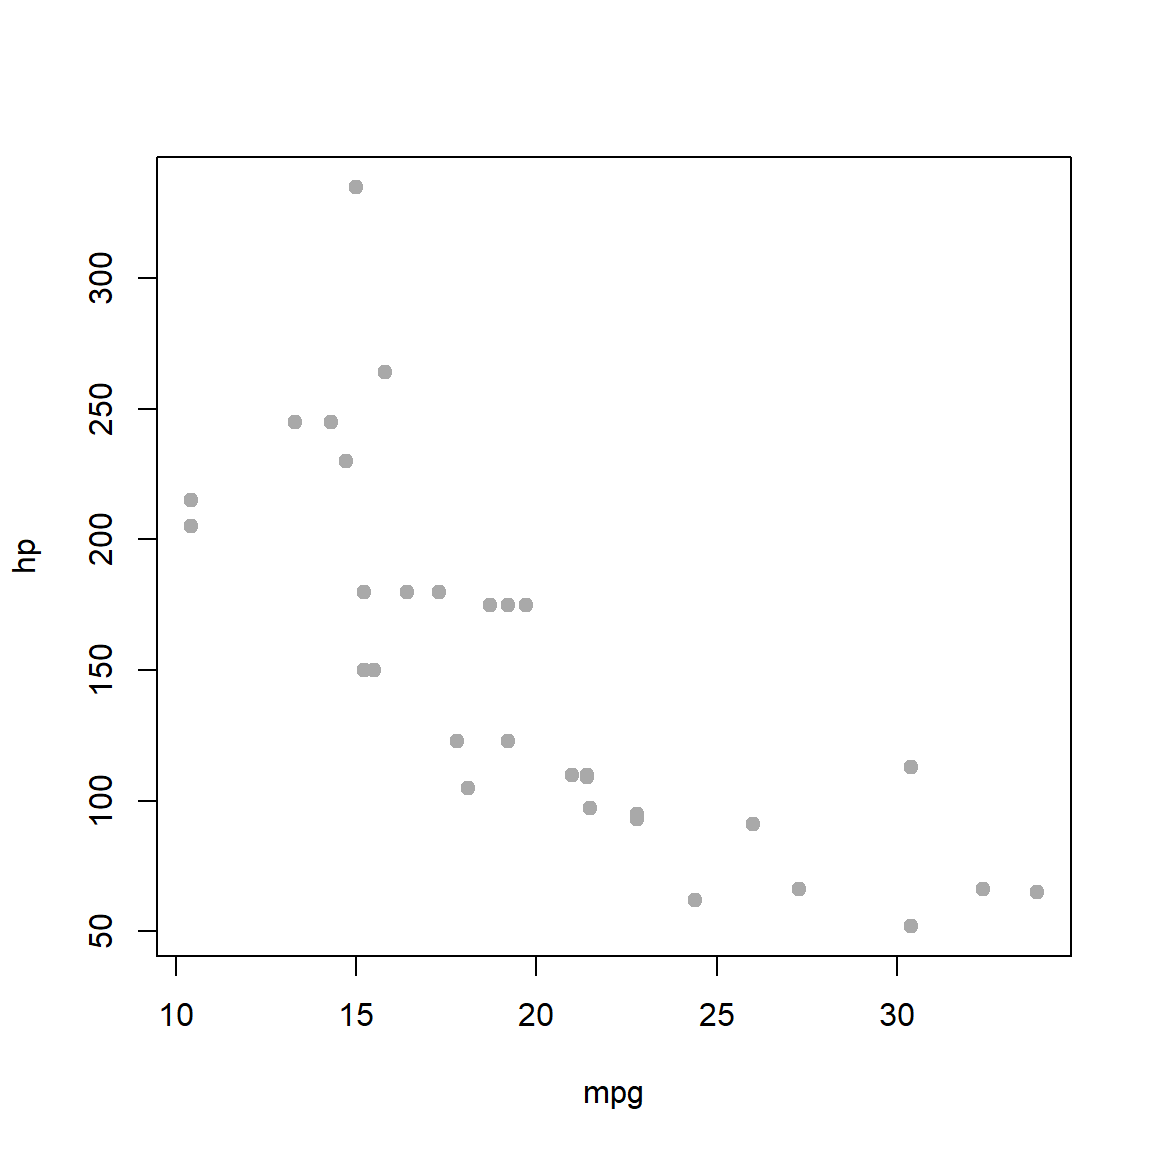
\includegraphics{StAndrewsTemplate_files/figure-latex/unnamed-chunk-25-1} \end{center}

\vspace{\baselineskip}

\hyperlink{tsk5}{\buttonT{Return to task on P\colpageref{sol5}}}
\eblockS
\hypertarget{sol6}{}
\bblockS[Solution]{\phantomsection\label{tsk6}6}
\bmp
\bblockST{Base R}

\begin{Shaded}
\begin{Highlighting}[]
\KeywordTok{plot}\NormalTok{(hp }\OperatorTok{~}\StringTok{ }\NormalTok{mpg, }\DataTypeTok{data =}\NormalTok{ mtcars,}
     \DataTypeTok{pch=}\DecValTok{19}\NormalTok{, }\DataTypeTok{col=}\StringTok{'darkgrey'}\NormalTok{)}
\end{Highlighting}
\end{Shaded}

\begin{center}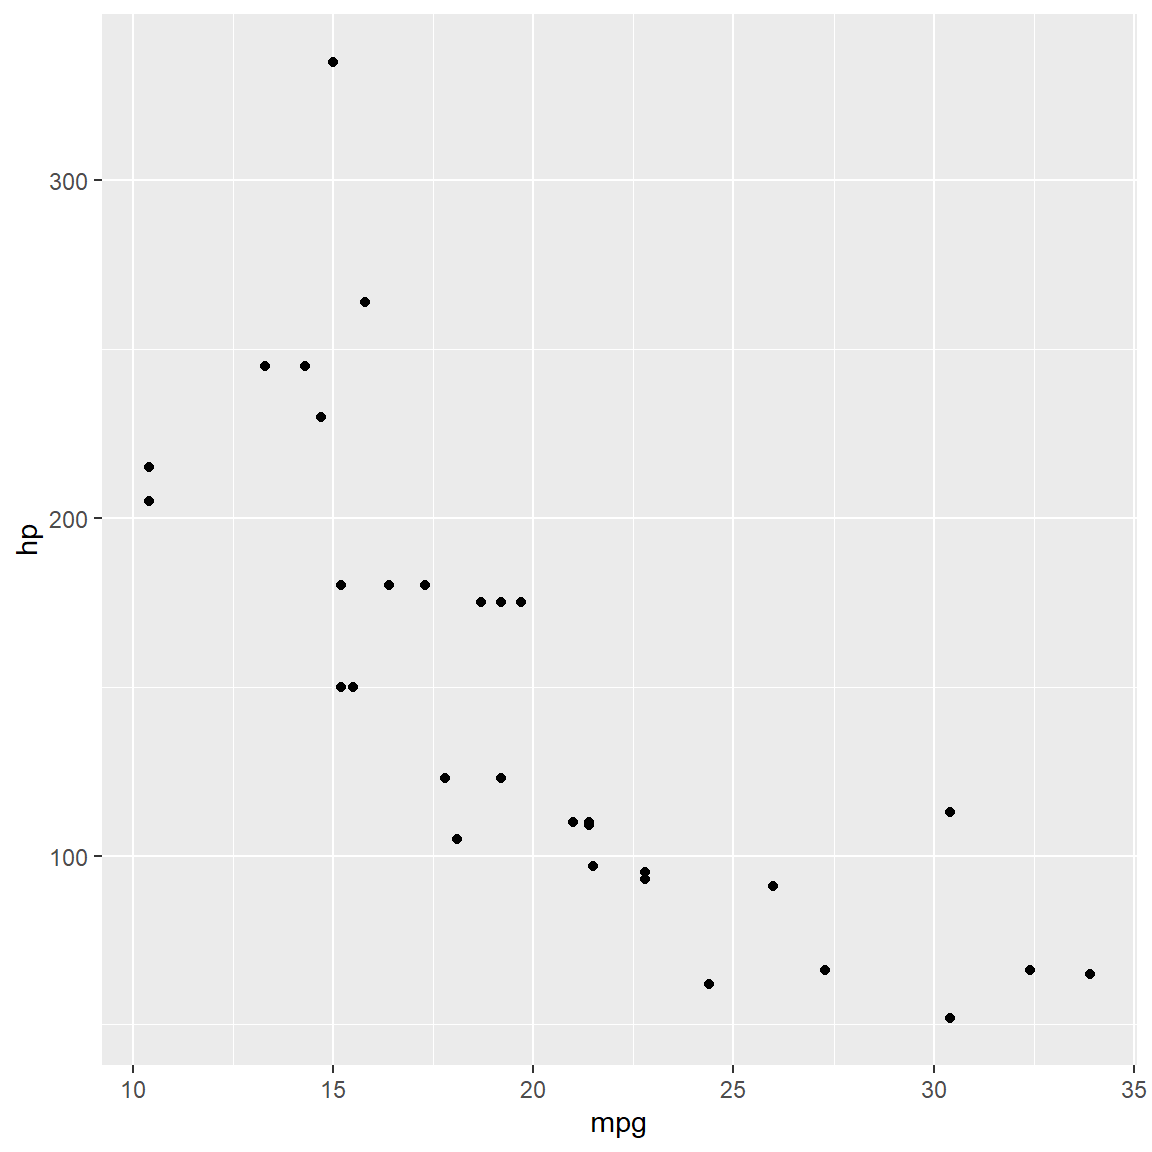
\includegraphics[width=0.6\linewidth]{StAndrewsTemplate_files/figure-latex/unnamed-chunk-26-1} \end{center}

The plot suggests that a linear relationship might exist between the two variables.
So we can proceed by fitting a linear model in R.

\eblockST
\emp
\hspace{0.01\textwidth}
\bmp\bblockST{tidyverse}

\begin{Shaded}
\begin{Highlighting}[]
\KeywordTok{ggplot}\NormalTok{(mtcars) }\OperatorTok{+}
\StringTok{    }\KeywordTok{geom_point}\NormalTok{(}\KeywordTok{aes}\NormalTok{(}\DataTypeTok{x =}\NormalTok{ mpg, }\DataTypeTok{y =}\NormalTok{ hp))}
\end{Highlighting}
\end{Shaded}

\begin{center}\includegraphics[width=0.6\linewidth]{StAndrewsTemplate_files/figure-latex/unnamed-chunk-27-1} \end{center}

The plot suggests that a linear relationship might exist between the two variables.
So we can proceed by fitting a linear model in R.

\eblockST
\emp

\vspace{\baselineskip}

\hyperlink{tsk6}{\buttonT{Return to task on P\colpageref{sol6}}}
\eblockS

  \bibliography{book.bib,packages.bib}

\printindex

\end{document}
